\section{Задание 1. Интегральная сумма}
\subsection{Интегральная сумма}
\subsection*{Задание}
Исследуйте интегральную сумму функции $ \frac{1}{1 + x^2} $,заданной на отрезке $ \left[-1;\sqrt{3}\right]$
\subsection*{Интегральная сумма функции на заданном отрезке в виде ступенчатой фигуры}
\begin{center}
	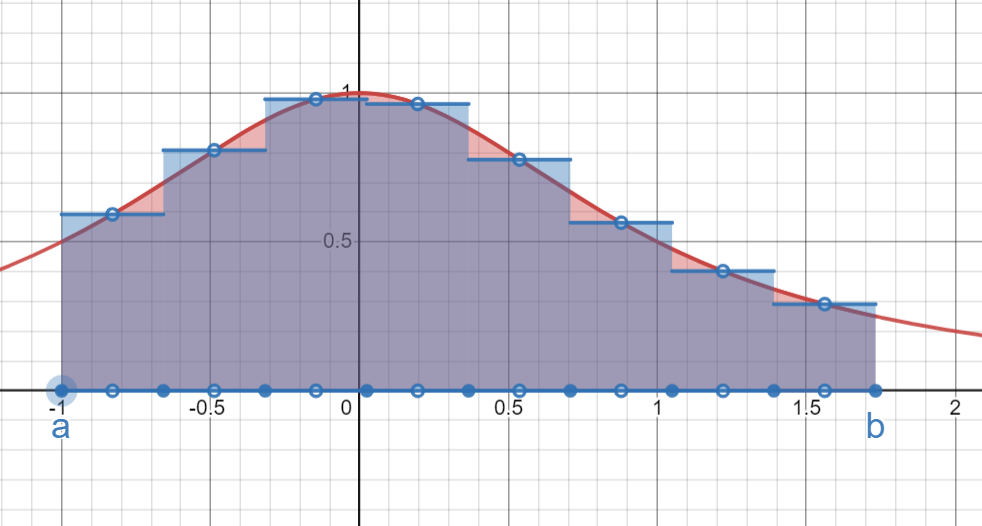
\includegraphics[width=0.4\linewidth]{task1/img1}\\
	\url{https://www.desmos.com/calculator/w21pp71fpr}
\end{center}
\subsection*{Исследование ступенчатой фигуры}
Рассмотрим разбиение на 3, 8 и 50 ступеней:
\begin{figure}[H]
	\centering
	\begin{subfigure}{0.3\textwidth}
		\centering
		\includegraphics[width=.8\linewidth]{task1/n3/left}\quad
		\caption*{Крайнее левое положение точек}
	\end{subfigure}
	\begin{subfigure}{0.3\textwidth}
		\centering
		\includegraphics[width=.8\linewidth]{task1/n3/middle}\quad
		\caption*{Промежуточное положение точек}
	\end{subfigure}
	\begin{subfigure}{0.3\textwidth}
		\centering
		\includegraphics[width=.8\linewidth]{task1/n3/right}\quad
		\caption*{Крайнее правое положение точек}
	\end{subfigure}
	\caption{Разбиение на 3 ступени}
\end{figure}

\begin{figure}[H]
	\centering
	\begin{subfigure}{0.3\textwidth}
		\centering
		\includegraphics[width=.8\linewidth]{task1/n8/left}\quad
		\caption*{Крайнее левое положение точек}
	\end{subfigure}
	\begin{subfigure}{0.3\textwidth}
		\centering
		\includegraphics[width=.8\linewidth]{task1/n8/middle}\quad
		\caption*{Промежуточное положение точек}
	\end{subfigure}
	\begin{subfigure}{0.3\textwidth}
		\centering
		\includegraphics[width=.8\linewidth]{task1/n8/right}\quad
		\caption*{Крайнее правое положение точек}
	\end{subfigure}
	\caption{Разбиение на 8 ступеней}
\end{figure}

\begin{figure}[H]
	\centering
	\begin{subfigure}{0.3\textwidth}
		\centering
		\includegraphics[width=.8\linewidth]{task1/n50/left}\quad
		\caption*{Крайнее левое положение точек}
	\end{subfigure}
	\begin{subfigure}{0.3\textwidth}
		\centering
		\includegraphics[width=.8\linewidth]{task1/n50/middle}\quad
		\caption*{Промежуточное положение точек}
	\end{subfigure}
	\begin{subfigure}{0.3\textwidth}
		\centering
		\includegraphics[width=.8\linewidth]{task1/n50/right}\quad
		\caption*{Крайнее правое положение точек}
	\end{subfigure}
	\caption{Разбиение на 50 ступеней}
\end{figure}
\subsection*{Заключение}
В процессе выполнения первой части первого задания были построены ступенчатые фигуры по графику. Ступенчатая фигура тем точнее, чем мельче разбиение и чем ближе выбранные точки к серединам разбиений
\subsection{Последовательность интегральных сумм}
\subsubsection*{Интегральная сумма}
\begin{figure}[H]
	\centering
	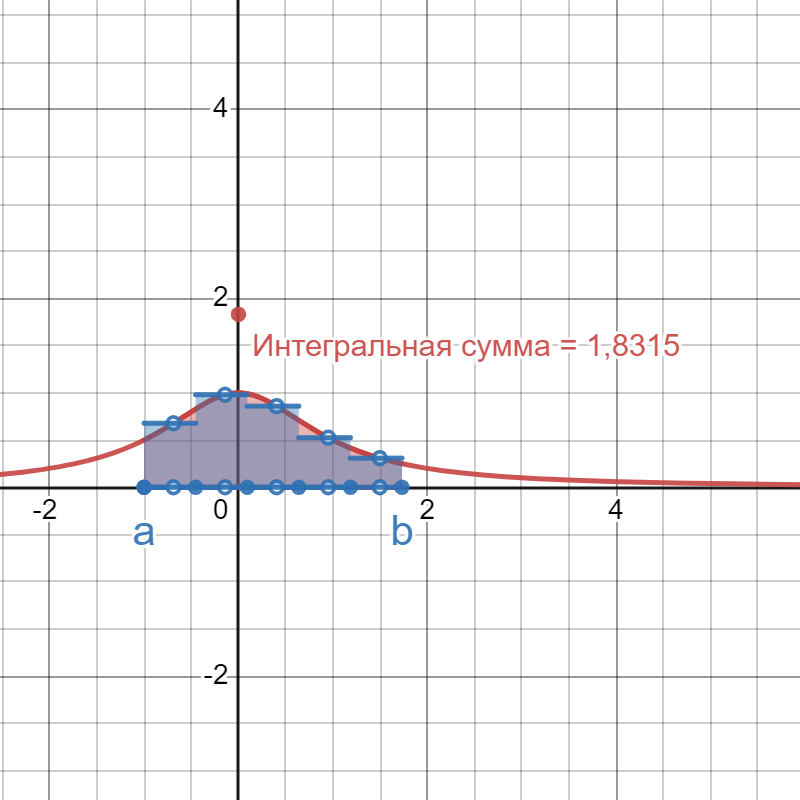
\includegraphics[width=0.4\linewidth]{task1/integrating_sums}\\
	\caption{Подсчет интегральной суммы}
\end{figure}
\subsubsection*{Исследование значения с ростом $ n $ при различных положениях точек}
\begin{figure}[H]
	\centering
	\begin{subfigure}{0.3\textwidth}
		\centering
		\includegraphics[width=.8\linewidth]{task1/sum_n3/left}\quad
		\caption*{Крайнее левое положение точек}
	\end{subfigure}
	\begin{subfigure}{0.3\textwidth}
		\centering
		\includegraphics[width=.8\linewidth]{task1/sum_n3/middle}\quad
		\caption*{Промежуточное положение точек}
	\end{subfigure}
	\begin{subfigure}{0.3\textwidth}
		\centering
		\includegraphics[width=.8\linewidth]{task1/sum_n3/right}\quad
		\caption*{Крайнее правое положение точек}
	\end{subfigure}
	\caption{Разбиение на 3 ступени}
\end{figure}

\begin{figure}[H]
	\centering
	\begin{subfigure}{0.3\textwidth}
		\centering
		\includegraphics[width=.8\linewidth]{task1/sum_n8/left}\quad
		\caption*{Крайнее левое положение точек}
	\end{subfigure}
	\begin{subfigure}{0.3\textwidth}
		\centering
		\includegraphics[width=.8\linewidth]{task1/sum_n8/middle}\quad
		\caption*{Промежуточное положение точек}
	\end{subfigure}
	\begin{subfigure}{0.3\textwidth}
		\centering
		\includegraphics[width=.8\linewidth]{task1/sum_n8/right}\quad
		\caption*{Крайнее правое положение точек}
	\end{subfigure}
	\caption{Разбиение на 8 ступеней}
\end{figure}

\begin{figure}[H]
	\centering
	\begin{subfigure}{0.3\textwidth}
		\centering
		\includegraphics[width=.8\linewidth]{task1/sum_n50/left}\quad
		\caption*{Крайнее левое положение точек}
	\end{subfigure}
	\begin{subfigure}{0.3\textwidth}
		\centering
		\includegraphics[width=.8\linewidth]{task1/sum_n50/middle}\quad
		\caption*{Промежуточное положение точек}
	\end{subfigure}
	\begin{subfigure}{0.3\textwidth}
		\centering
		\includegraphics[width=.8\linewidth]{task1/sum_n50/right}\quad
		\caption*{Крайнее правое положение точек}
	\end{subfigure}
	\caption{Разбиение на 50 ступеней}
\end{figure}
\subsubsection*{Аналитическое вычисление интеграла}
\begin{equation*}
	\int_{-1}^{\sqrt{3}}\frac{dx}{1+x^2}=\arctg{x\bigg|_{-1}^{\sqrt{3}}}=\frac{\pi }{3}-\left(-\frac{\pi }{4}\right)=\frac{7\pi}{12}\approxeq1,8326
\end{equation*}
Интегральная сумма тем точнее, чем мельче разбиение и чем ближе выбранные точки к серединам разбиений
\subsubsection*{Последовательность интегральных сумм}
\begin{figure}[H]
	\centering
	\begin{subfigure}{0.3\textwidth}
		\centering
		\includegraphics[width=.8\linewidth]{task1/sums/left}\quad
		\caption*{Крайнее левое положение точек}
	\end{subfigure}
	\begin{subfigure}{0.3\textwidth}
		\centering
		\includegraphics[width=.8\linewidth]{task1/sums/middle}\quad
		\caption*{Промежуточное положение точек}
	\end{subfigure}
	\begin{subfigure}{0.3\textwidth}
		\centering
		\includegraphics[width=.8\linewidth]{task1/sums/right}\quad
		\caption*{Крайнее правое положение точек}
	\end{subfigure}
	\caption{Зависимость от расположения точек}
	\url{https://www.desmos.com/calculator/zrwq9vbkt0}
\end{figure}
\subsubsection*{Заключение}
В процессе выполнения части 2 задания 1 были сравнены значения интегральных сумм и аналитического исчисления. Можно сделать вывод, что вычисление определенного интеграла достаточно точное и его точность прямо пропорциональна количеству точек, которые мы выбираем и их близость к середине разбиений



